\section{nlist Strukturreferenz}
\label{structnlist}\index{nlist@{nlist}}
{\tt \#include $<$linklist.h$>$}

Zusammengeh\"{o}rigkeiten von nlist:\begin{figure}[H]
\begin{center}
\leavevmode
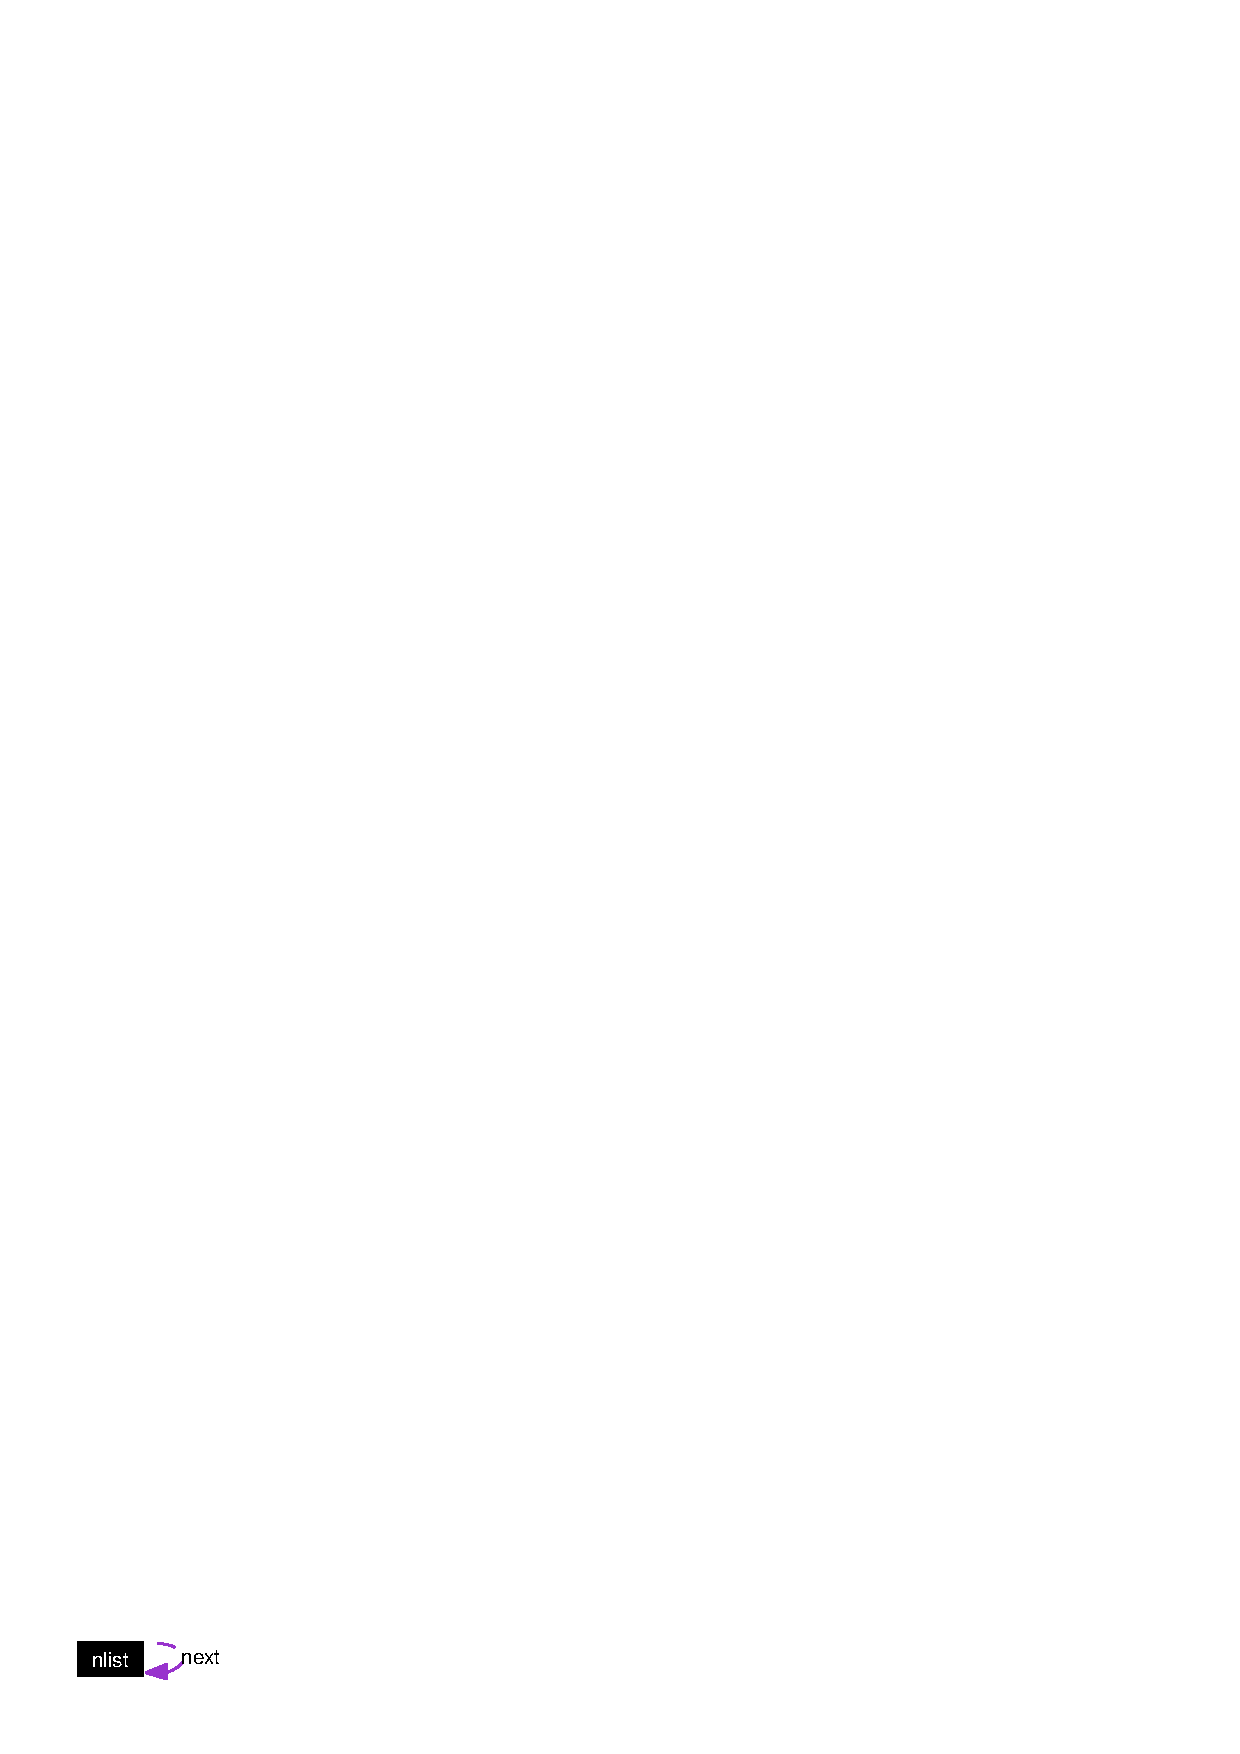
\includegraphics[width=54pt]{structnlist__coll__graph}
\end{center}
\end{figure}
\subsection*{Datenfelder}
\begin{CompactItemize}
\item 
char {\bf string} [80]
\item 
{\bf nlist} $\ast$ {\bf next}
\end{CompactItemize}


\subsection{Ausf\"{u}hrliche Beschreibung}




Definiert in Zeile 4 der Datei linklist.h.

\subsection{Dokumentation der Datenelemente}
\index{nlist@{nlist}!next@{next}}
\index{next@{next}!nlist@{nlist}}
\subsubsection{\setlength{\rightskip}{0pt plus 5cm}struct {\bf nlist}$\ast$ {\bf nlist::next}}\label{structnlist_6e5fbb2f12a2799e60611dbda92c6f38}




Definiert in Zeile 5 der Datei linklist.h.

Wird benutzt von add\_\-nlist(), del\_\-nlist(), isinlist(), new\_\-nlist(), write\_\-html\_\-head() und write\_\-html\_\-tail().\index{nlist@{nlist}!string@{string}}
\index{string@{string}!nlist@{nlist}}
\subsubsection{\setlength{\rightskip}{0pt plus 5cm}char {\bf nlist::string}[80]}\label{structnlist_272774fb3950796b85497317de3dd85a}




Definiert in Zeile 4 der Datei linklist.h.

Wird benutzt von isinlist(), new\_\-nlist(), write\_\-html\_\-head() und write\_\-html\_\-tail().

Die Dokumentation f\"{u}r diese Struktur wurde erzeugt aufgrund der Datei:\begin{CompactItemize}
\item 
oosalizer/{\bf linklist.h}\end{CompactItemize}
